\documentclass[11pt]{article}

% ====================================================
% PACKAGES
% ====================================================
\usepackage[margin=1in, headheight=13.6pt]{geometry}
\usepackage[T1]{fontenc}
\usepackage{lmodern}
\usepackage{microtype}
\usepackage{setspace}
\usepackage{tcolorbox}
\usepackage{amsmath, amssymb, mathtools}
\usepackage{siunitx}

\usepackage{graphicx}
\usepackage{float}
\usepackage{subcaption}

\usepackage{enumitem}
\usepackage{booktabs}
\usepackage{longtable}
\usepackage{array}
\usepackage{multirow}

\usepackage{xcolor}
\usepackage{hyperref}

\usepackage{fancyhdr}
\usepackage{lastpage}

\usepackage{listings}
\usepackage{indentfirst}
\usepackage[justification=centering]{caption}

% Python source style for \CodeListing
\lstdefinestyle{pystyle}{
    language=Python,
    basicstyle=\ttfamily\footnotesize,
    keywordstyle=\color{blue!60!black}\bfseries,
    stringstyle=\color{orange!70!black},
    commentstyle=\color{gray!60!black}\itshape,
    numbers=left,
    numberstyle=\tiny\color{gray!70},
    numbersep=8pt,
    breaklines=true,
    showstringspaces=false,
    frame=single,
    rulecolor=\color{gray!40},
    tabsize=4,
    columns=fullflexible,
    captionpos=b,
    literate={°}{{\textdegree}}1,
}
\lstset{style=pystyle}

\pagestyle{fancy}
\fancyhf{}
\lhead{\Assignment\ |\ \course}
\rhead{\Name\ |\ \today}
\cfoot{Page \thepage\ of~\pageref{LastPage}}

\hypersetup{
    colorlinks,
    linkcolor={red!50!black},
    citecolor={blue!50!black},
    urlcolor={blue!80!black}
}

\newcommand{\Name}{Arael Anaya}
\newcommand{\Assignment}{Exam 2}
\newcommand{\course}{Advanced Dynamics}

% Boxed final-answer environment
\newtcolorbox{result}{
    colback=blue!3!white,
    colframe=blue!40!black,
    boxrule=0.6pt,
    arc=2pt,
    left=6pt, right=6pt, top=4pt, bottom=4pt
}

% Code listing: sources the .py file directly.
\newcommand{\CodeListing}[3]{%
\IfFileExists{#1}%
    {\lstinputlisting[style=pystyle,caption={#2},label={#3}]{#1}}%
    {\begin{quote}\itshape Source file \texttt{#1} not found yet; this
        listing will populate automatically once the file is written.\end{quote}}}

\begin{document}

% ====================================================
% PROBLEM 1
% ====================================================
\section*{Problem 1}

\begin{figure}[H]
    \centering
    
\includegraphics[width=0.55\linewidth]{Figures/Problem Set/Problem 1.png}
\end{figure}

A bar of mass $m$, length $\ell$ is welded to a bar of mass $2m$, length $2\ell$ to form the T shown. The body is pinned to a post that rotates at the constant rate $\Omega$.

The moment of inertia tensor for the T-shaped bar is given by,
$$I = \begin{bmatrix} \tfrac{1}{12}m\ell^2 & 0 & 0 \\ 0 & \tfrac{20}{3}m\ell^2 & 0 \\ 0 & 0 & \tfrac{27}{4}m\ell^2\end{bmatrix},$$
in the body frame $\{\hat b\}$ along the principal axes of the body, centered at the pivot point, with $\hat b_1$ pointing along the length-$2\ell$ bar (down and to the right), $\hat b_2$ pointing up and to the right parallel to the length-$\ell$ bar, and $\hat b_3$ pointing out of the page.

\begin{enumerate}[label=(\alph*)]
    \item Calculate the angular velocity $\omega$ and angular momentum $H$ of the pendulum, each expressed in the body frame.

    Let $\hat n_2$ be the vertical spin axis of the post, fixed in the inertial frame, so $\vec\Omega=\Omega\,\hat n_2$.
    $$\hat n_2 = -\cos\theta\,\hat b_1+\sin\theta\,\hat b_2$$
    $$\vec\omega = \Omega\,\hat n_2+\dot\theta\,\hat b_3 = -\Omega\cos\theta\,\hat b_1+\Omega\sin\theta\,\hat b_2+\dot\theta\,\hat b_3$$
    $$\boxed{\vec H = I\vec\omega = -\frac{1}{12}m\ell^2\Omega\cos\theta\,\hat b_1+\frac{20}{3}m\ell^2\Omega\sin\theta\,\hat b_2+\frac{27}{4}m\ell^2\dot\theta\,\hat b_3}$$
    $$\boxed{{}^B\frac{d\vec H}{dt} = \frac{1}{12}m\ell^2\Omega\dot\theta\sin\theta\,\hat b_1+\frac{20}{3}m\ell^2\Omega\dot\theta\cos\theta\,\hat b_2+\frac{27}{4}m\ell^2\ddot\theta\,\hat b_3}$$

    \item Calculate the rate of change of angular momentum, ${}^N\dfrac{dH}{dt}$.

    $${}^N\frac{d\vec H}{dt} = {}^B\frac{d\vec H}{dt}+\vec\omega\times\vec H$$
    $$\boxed{{}^N\frac{d\vec H}{dt} = \frac{1}{6}m\ell^2\Omega\dot\theta\sin\theta\,\hat b_1+\frac{40}{3}m\ell^2\Omega\dot\theta\cos\theta\,\hat b_2+\left(\frac{27}{4}m\ell^2\ddot\theta-\frac{79}{12}m\ell^2\Omega^2\sin\theta\cos\theta\right)\hat b_3}$$

    \item Compute the applied moment due to gravity, treating that moment as two forces applied at the center of mass of each bar. Note that there is also a torque applied about the vertical axis to keep the shaft spinning at a constant rate $\Omega$.

    $\vec r_{2m}=\ell\,\hat b_1$, $\vec r_m=2\ell\,\hat b_1$, $\hat g=\cos\theta\,\hat b_1-\sin\theta\,\hat b_2$:
    $$\vec F_{2m} = 2mg\cos\theta\,\hat b_1-2mg\sin\theta\,\hat b_2, \qquad \vec F_{m} = mg\cos\theta\,\hat b_1-mg\sin\theta\,\hat b_2$$
    $$\sum\vec M = \ell\hat b_1\times\vec F_{2m}+2\ell\hat b_1\times\vec F_m = -2\ell mg\sin\theta\,\hat b_3-2\ell mg\sin\theta\,\hat b_3$$
    $$\boxed{\sum\vec M = -4mg\ell\sin\theta\,\hat b_3}$$
    (The $\hat b_1,\hat b_2$ components of part (b) are balanced by the pin/motor reaction.) Only the $\hat b_3$ component is used in the equation of motion because the pin axis is $\hat b_3$, and the motor torque needed to hold $\Omega$ constant acts about the vertical axis, which lies entirely in the $\hat b_1$-$\hat b_2$ plane, so $\hat b_3$ is the only component of the moment equation free of an unknown reaction/motor torque.

    \item Find the equation of motion for $\theta$, using ${}^N\dfrac{dH}{dt}=\Sigma M$. At what critical value of $\Omega$ does a bifurcation occur?

    $$-4mg\ell\sin\theta = \frac{27}{4}m\ell^2\ddot\theta-\frac{79}{12}m\ell^2\Omega^2\sin\theta\cos\theta$$
    $$\boxed{\ddot\theta = \frac{79}{81}\Omega^2\sin\theta\cos\theta-\frac{16}{27}\frac{g}{\ell}\sin\theta}$$
    Small $\theta$:
    $$\boxed{\ddot\theta \approx \left(\frac{79}{81}\Omega^2-\frac{16}{27}\frac{g}{\ell}\right)\theta}$$
    Bifurcation when the coefficient vanishes:
    $$\frac{79}{81}\Omega^2 = \frac{16}{27}\frac{g}{\ell} \quad\Longrightarrow\quad \boxed{\Omega_{crit}=\sqrt{\frac{48}{79}\frac{g}{\ell}}}$$
    This is a pitchfork bifurcation: for $\Omega<\Omega_{crit}$, $\theta=0$ is the only equilibrium and it's stable, while for $\Omega>\Omega_{crit}$ it loses stability and two new symmetric equilibria appear at $\theta=\pm\arccos(\Omega_{crit}^2/\Omega^2)$ (the full nonlinear $\ddot\theta=0$ roots), consistent with the sign-flip of the linearized coefficient above.

    \item Plot the phase portrait before and after $\Omega_{crit}$.

    $\theta_1=\theta$, $\theta_2=\dot\theta$:
    $$\begin{cases}\dot\theta_1 = \theta_2\\[4pt] \dot\theta_2 = \dfrac{79}{81}\Omega^2\sin\theta_1\cos\theta_1-\dfrac{16}{27}\dfrac{g}{\ell}\sin\theta_1\end{cases}$$
    $$\boxed{J = \begin{bmatrix}0 & 1\\[4pt] \dfrac{79}{81}\Omega^2\cos2\theta_1-\dfrac{16}{27}\dfrac{g}{\ell}\cos\theta_1 & 0\end{bmatrix}}$$
    At $\theta_1=0$: $J_{21}=\tfrac{79}{81}\Omega^2-\tfrac{16}{27}\tfrac{g}{\ell}$, giving imaginary eigenvalues (center) for $\Omega<\Omega_{crit}$, real opposite-sign (saddle) for $\Omega>\Omega_{crit}$.

    \begin{figure}[H]
        \centering
        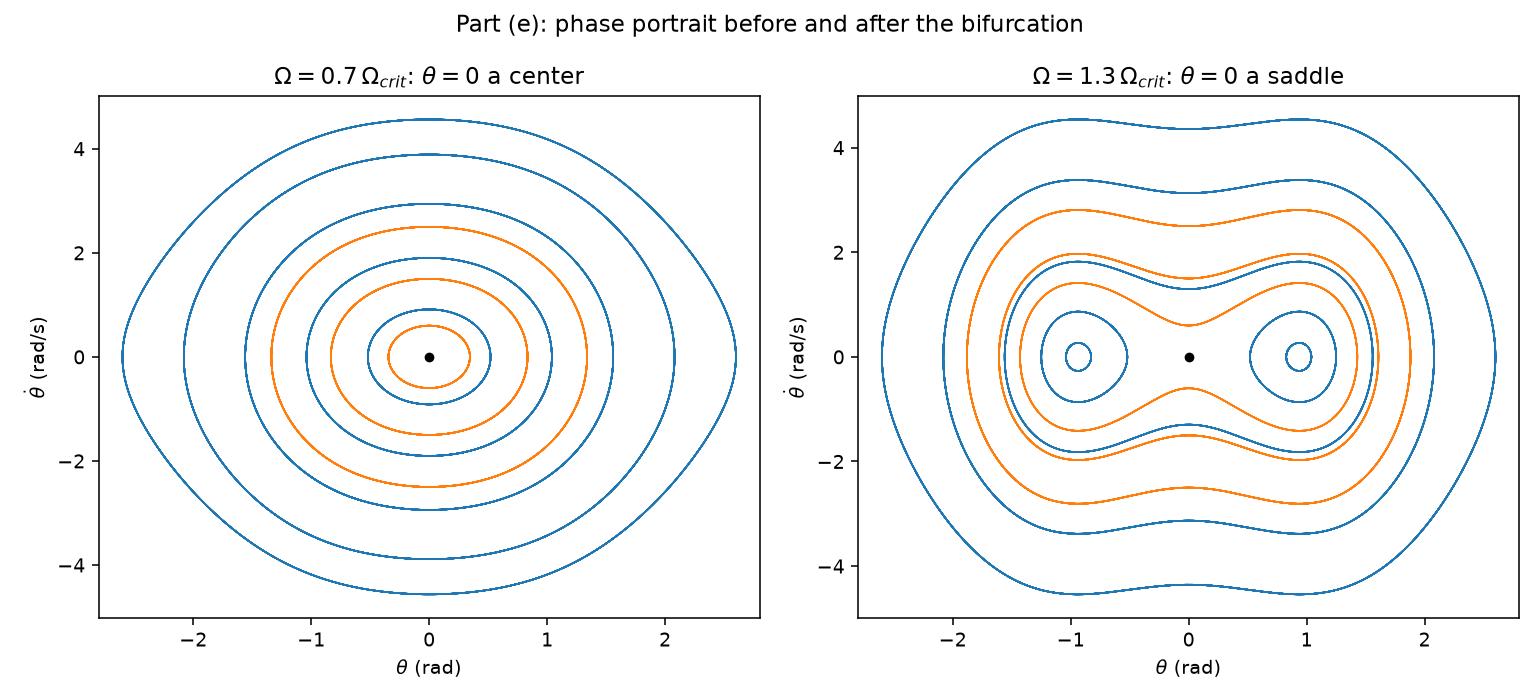
\includegraphics[width=\linewidth]{Figures/Graphs/Problem1/partE_phase_portrait.png}
        \caption{Phase portraits at $\Omega=0.7\,\Omega_{crit}$ and $1.3\,\Omega_{crit}$ ($\ell=1$, $g=9.81$). Below $\Omega_{crit}$: single center at $\theta=0$. Above: pitchfork into a saddle and two centers at $\theta=\pm\arccos(\Omega_{crit}^2/\Omega^2)$.}
    \end{figure}

\end{enumerate}

% ====================================================
% PROBLEM 2
% ====================================================
\newpage
\section*{Problem 2}

\begin{figure}[H]
    \centering
    
\includegraphics[width=0.62\linewidth]{Figures/Problem Set/Problem 2.png}
\end{figure}

Consider a coin rolling along its edge on a flat surface. To describe its orientation, we consider the position of the center of the coin to be defined as,
$$\vec r_c = x\hat n_1+y\hat n_2+z\hat n_3.$$

To describe its orientation, we use 3-1-3 Euler angles, just as in HW6. Consider the Euler angles to be:

First, imagine the coin to be laying flat on the ground. Rotate the heading of the coin by a counterclockwise angle $\psi$ around the $\hat n_3$ axis. Second, rotate the coin upward through the angle $\theta$. If $\theta=90^\circ$, the coin is standing on its edge, pointing in the direction of $\hat b_1$. Finally, we consider rolling around the $\hat b_3=\hat b_3''$ axis by the angle $\phi$.

\textit{Note: If you're having a hard time understanding the orientation of the coin, feel free to reach out! I'll try to re-describe this orientation.}

\begin{enumerate}[label=(\alph*)]
    \item Briefly, re-derive both the cosine matrix and angular velocity of the coin using the angles given (you can bring this in from HW6, and the angle definitions should match this assignment).

    $3$-$1$-$3$ rotation matrices:
    $$R(\psi)=\begin{bmatrix}\cos\psi&\sin\psi&0\\-\sin\psi&\cos\psi&0\\0&0&1\end{bmatrix}, \quad R(\theta)=\begin{bmatrix}1&0&0\\0&\cos\theta&\sin\theta\\0&-\sin\theta&\cos\theta\end{bmatrix}, \quad R(\phi)=\begin{bmatrix}\cos\phi&\sin\phi&0\\-\sin\phi&\cos\phi&0\\0&0&1\end{bmatrix}$$
    $C=R(\phi)R(\theta)R(\psi)$:
    $$R(\theta)R(\psi)=\begin{bmatrix}\cos\psi & \sin\psi & 0\\-\sin\psi\cos\theta & \cos\psi\cos\theta & \sin\theta\\\sin\psi\sin\theta & -\cos\psi\sin\theta & \cos\theta\end{bmatrix}$$
    $$\boxed{C=\begin{bmatrix}
    \cos\psi\cos\phi-\sin\psi\cos\theta\sin\phi & \sin\psi\cos\phi+\cos\psi\cos\theta\sin\phi & \sin\theta\sin\phi\\[4pt]
    -\cos\psi\sin\phi-\sin\psi\cos\theta\cos\phi & -\sin\psi\sin\phi+\cos\psi\cos\theta\cos\phi & \sin\theta\cos\phi\\[4pt]
    \sin\psi\sin\theta & -\cos\psi\sin\theta & \cos\theta
    \end{bmatrix}}$$

    $$\vec\omega = \dot\psi\,\hat n_3+\dot\theta\,\hat b_1'+\dot\phi\,\hat b_3$$
    Note $\hat n_3=\hat b_3'$ (the first rotation is about $\hat n_3$, so it is unchanged by that rotation), not $\hat b_3''$. Expanding $\hat b_3'$ in the $\{\hat b''\}$ basis using $R(\theta)$:
    $$\hat n_3 = \hat b_3' = \sin\theta\,\hat b_2''+\cos\theta\,\hat b_3''$$
    With $\hat b_3''=\hat b_3$, $\hat b_2''=\sin\phi\,\hat b_1+\cos\phi\,\hat b_2$, $\hat b_1'=\cos\phi\,\hat b_1-\sin\phi\,\hat b_2$:
    $$\boxed{\vec\omega = (\dot\theta\cos\phi+\dot\psi\sin\theta\sin\phi)\,\hat b_1+(-\dot\theta\sin\phi+\dot\psi\sin\theta\cos\phi)\,\hat b_2+(\dot\phi+\dot\psi\cos\theta)\,\hat b_3}$$

    \item The coordinate $z$ can be defined geometrically from one or more Euler angles. What is that relationship?

    $$\boxed{z = r\sin\theta} \quad\Longrightarrow\quad \dot z = r\cos\theta\,\dot\theta$$

    \item Choosing $(x,y,\psi,\theta,\phi)$ as your five degrees of freedom, derive the Lagrangian function, $\mathcal L$.

    $I_1=I_2\equiv I_t=\tfrac14Mr^2$, $I_3\equiv I_a=\tfrac12Mr^2$:
    $$\omega_1^2+\omega_2^2 = \dot\theta^2+\dot\psi^2\sin^2\theta, \qquad \omega_3^2 = \dot\phi^2+2\dot\phi\dot\psi\cos\theta+\dot\psi^2\cos^2\theta$$
    $$T = \underbrace{\tfrac12M\left(\dot x^2+\dot y^2+r^2\cos^2\theta\,\dot\theta^2\right)}_{T_{trans}}+\underbrace{\tfrac18Mr^2\left(\dot\theta^2+\dot\psi^2\sin^2\theta\right)+\tfrac14Mr^2\left(\dot\phi^2+2\dot\phi\dot\psi\cos\theta+\dot\psi^2\cos^2\theta\right)}_{T_{rot}}$$
    $$\boxed{V = Mgr\sin\theta}$$
    $$\boxed{\begin{aligned}\mathcal L = T-V = \tfrac12M\Big(\dot x^2+\dot y^2&+r^2\cos^2\theta\,\dot\theta^2\Big)+\tfrac18Mr^2\left(\dot\theta^2+\dot\psi^2\sin^2\theta\right)\\ &+\tfrac14Mr^2\left(\dot\phi^2+2\dot\phi\dot\psi\cos\theta+\dot\psi^2\cos^2\theta\right)-Mgr\sin\theta\end{aligned}}$$

    \item There are two non-holonomic constraints on the velocity of the point that touches the ground, both the no-slip condition and a knife-edge constraint. The third constraint in the $z$-direction (that it stays on the ground) was taken care of in part (b). These can be taken together as the constraint, $\vec v_A = \vec 0$.

    Let $\vec v_A = \vec v_C + \vec\omega\times\vec r_{A/C}$, where $\vec r_{A/C}$ is the position of $A$ with respect to $C$. Derive the constraints in the $x$ and $y$ direction.

    $\vec r_{A/C}=-r\hat b_2''$ (fixed in $\{\hat b''\}$, before spin), with $C''=R(\theta)R(\psi)$ and
    $$\vec\omega = \dot\theta\,\hat b_1''+\dot\psi\sin\theta\,\hat b_2''+(\dot\phi+\dot\psi\cos\theta)\,\hat b_3''$$
    $$\vec\omega\times\vec r_{A/C} = r(\dot\phi+\dot\psi\cos\theta)\,\hat b_1''-r\dot\theta\,\hat b_3''$$
    ${}^N\vec V_C=-\vec\omega\times\vec r_{A/C}$, rotated into $\{\hat n\}$ by $(C'')^T$:
    $$\dot x = -r(\dot\phi+\dot\psi\cos\theta)\cos\psi+r\dot\theta\sin\theta\sin\psi, \qquad \dot y = -r(\dot\phi+\dot\psi\cos\theta)\sin\psi-r\dot\theta\sin\theta\cos\psi$$
    Pfaffian form $\phi_j=\sum_i a_{ji}\dot q_i=0$, $q=(x,y,\theta,\psi,\phi)$:
    $$a_{1x}=1,\ a_{1y}=0,\ a_{1\theta}=-r\sin\psi\sin\theta,\ a_{1\psi}=r\cos\psi\cos\theta,\ a_{1\phi}=r\cos\psi$$
    $$a_{2x}=0,\ a_{2y}=1,\ a_{2\theta}=r\sin\theta\cos\psi,\ a_{2\psi}=r\sin\psi\cos\theta,\ a_{2\phi}=r\sin\psi$$
    $$\boxed{\phi_1=\dot x-r\sin\theta\sin\psi\,\dot\theta+r\cos\theta\cos\psi\,\dot\psi+r\cos\psi\,\dot\phi=0}$$
    $$\boxed{\phi_2=\dot y+r\sin\theta\cos\psi\,\dot\theta+r\cos\theta\sin\psi\,\dot\psi+r\sin\psi\,\dot\phi=0}$$

    \item Construct the matrix equation $A\ddot y = b$, where $y = [\dot x,\dot y,\dot\psi,\dot\theta,\dot\phi,\ddot x,\ddot y,\ddot\psi,\ddot\theta,\ddot\phi,\lambda_1,\lambda_2]^T$. The matrix $A$ and vector $b$ will depend on any of the state variables in the system.

    As posed, $y$ is the assembled first-order form: with $\dot q=(\dot x,\dot y,\dot\psi,\dot\theta,\dot\phi)$, $\ddot q=(\ddot x,\ddot y,\ddot\psi,\ddot\theta,\ddot\phi)$, and $\lambda=(\lambda_1,\lambda_2)$, the $12\times12$ system is the block equation
    $$\begin{bmatrix} I_5 & 0_{5\times7}\\[2pt] 0_{7\times5} & A_7\end{bmatrix}\begin{bmatrix}\dot q\\ \ddot q\\ \lambda\end{bmatrix} = \begin{bmatrix}\dot q\\ b_7\end{bmatrix},$$
    where the top $5$ rows are just an identity block that carries the already-known $\dot q$ straight through, so that one solve returns the entire state derivative $(\dot q,\ddot q)$ together with $\lambda$; the bottom $7$ rows are the genuine dynamics, the $7\times7$ system $A_7\ddot q_\lambda=b_7$ (with $\ddot q_\lambda=(\ddot q,\lambda)$) derived below. Because the top block is trivial, it's the $7\times7$ block $A_7,b_7$ that is actually assembled and solved each time step (\texttt{build\_system}, Appendix~\ref{lst:p2}).

    $$\frac{d}{dt}\left(\frac{\partial\mathcal L}{\partial\dot q_i}\right)-\frac{\partial\mathcal L}{\partial q_i} = \lambda_1 a_{1i}+\lambda_2 a_{2i}$$
    $$\boxed{\begin{aligned}
    x:&\quad M\ddot x = \lambda_1\\
    y:&\quad M\ddot y = \lambda_2\\
    \psi:&\quad Mr^2\left[\tfrac14\left(\cos^2\theta+1\right)\ddot\psi+\tfrac12\cos\theta\,\ddot\phi-\tfrac12\sin\theta\,\dot\theta\left(\dot\phi+\dot\psi\cos\theta\right)\right] = r\cos\theta\left(\lambda_1\cos\psi+\lambda_2\sin\psi\right)\\
    \theta:&\quad Mr^2\left(\cos^2\theta+\tfrac14\right)\ddot\theta+Mr^2\sin\theta\cos\theta\left(\tfrac14\dot\psi^2-\dot\theta^2\right)+\tfrac12Mr^2\sin\theta\,\dot\phi\dot\psi+Mgr\cos\theta \\ &\hspace{7cm}= r\sin\theta\left(\lambda_2\cos\psi-\lambda_1\sin\psi\right)\\
    \phi:&\quad \tfrac12Mr^2\left(\ddot\phi+\ddot\psi\cos\theta-\dot\psi\dot\theta\sin\theta\right) = r\left(\lambda_1\cos\psi+\lambda_2\sin\psi\right)
    \end{aligned}}$$
    Differentiating $\phi_1,\phi_2$ once:
    $$\boxed{\ddot x-r\sin\theta\sin\psi\,\ddot\theta+r\cos\theta\cos\psi\,\ddot\psi+r\cos\psi\,\ddot\phi = r\cos\theta\sin\psi(\dot\theta^2+\dot\psi^2)+2r\sin\theta\cos\psi\,\dot\theta\dot\psi+r\sin\psi\,\dot\phi\dot\psi}$$
    $$\boxed{\ddot y+r\sin\theta\cos\psi\,\ddot\theta+r\cos\theta\sin\psi\,\ddot\psi+r\sin\psi\,\ddot\phi = -r\cos\theta\cos\psi(\dot\theta^2+\dot\psi^2)+2r\sin\theta\sin\psi\,\dot\theta\dot\psi-r\cos\psi\,\dot\phi\dot\psi}$$
    This gives $7$ equations in the $7$ unknowns $\ddot q_\lambda=(\ddot x,\ddot y,\ddot\psi,\ddot\theta,\ddot\phi,\lambda_1,\lambda_2)$. Writing them as $A_7\ddot q_\lambda=b_7$ with that ordering, matching the professor's $(\psi,\theta)$ order rather than $(\theta,\psi)$ (shorthand $c_\theta=\cos\theta$, $s_\theta=\sin\theta$, $c_\psi=\cos\psi$, $s_\psi=\sin\psi$; all unlabeled entries are $0$):
    $$\resizebox{\textwidth}{!}{$A_7=\begin{bmatrix}
    M & 0 & 0 & 0 & 0 & -1 & 0\\
    0 & M & 0 & 0 & 0 & 0 & -1\\
    0 & 0 & \tfrac14Mr^2\!\left(c_\theta^2+1\right) & 0 & \tfrac12Mr^2c_\theta & -rc_\theta c_\psi & -rc_\theta s_\psi\\
    0 & 0 & 0 & Mr^2\!\left(c_\theta^2+\tfrac14\right) & 0 & rs_\theta s_\psi & -rs_\theta c_\psi\\
    0 & 0 & \tfrac12Mr^2c_\theta & 0 & \tfrac12Mr^2 & -rc_\psi & -rs_\psi\\
    1 & 0 & rc_\psi c_\theta & -rs_\psi s_\theta & rc_\psi & 0 & 0\\
    0 & 1 & rs_\psi c_\theta & rs_\theta c_\psi & rs_\psi & 0 & 0
    \end{bmatrix}$}$$
    $$\resizebox{0.7\textwidth}{!}{$b_7=\begin{bmatrix}
    0\\[2pt] 0\\[2pt]
    \tfrac12Mr^2s_\theta\dot\theta\left(\dot\phi+\dot\psi c_\theta\right)\\[4pt]
    -Mr^2 s_\theta c_\theta\!\left(\tfrac14\dot\psi^2-\dot\theta^2\right)-\tfrac12Mr^2s_\theta\dot\phi\dot\psi-Mgr c_\theta\\[4pt]
    \tfrac12Mr^2\dot\psi\dot\theta s_\theta\\[4pt]
    rs_\psi c_\theta\!\left(\dot\psi^2+\dot\theta^2\right)+rs_\psi\dot\phi\dot\psi+2rs_\theta c_\psi\dot\psi\dot\theta\\[4pt]
    2rs_\psi s_\theta\dot\psi\dot\theta-rc_\psi c_\theta\!\left(\dot\psi^2+\dot\theta^2\right)-rc_\psi\dot\phi\dot\psi
    \end{bmatrix}$}$$
    with rows/columns ordered $(\ddot x,\ddot y,\ddot\psi,\ddot\theta,\ddot\phi,\lambda_1,\lambda_2)$; rows 1--2 are the $x,y$ equations, rows 3--5 are the $\psi,\theta,\phi$ equations above, and rows 6--7 are the differentiated constraints $\dot\phi_1=0$, $\dot\phi_2=0$.

    \item Using this matrix equation to numerically solve your equations of motion. Choose a reasonable mass and radius, and choose an initial condition with $\theta_0\neq0$ and $\dot\psi_0\neq0$, and choose $\dot x_0,\dot y_0$ based on your equations of constraint. Otherwise choose initial conditions equal to $0$.

    $r=1$, $M=1$; $\theta_0=1.2$, $\psi_0=\phi_0=0$, $\dot\theta_0=0$, $\dot\psi_0=1.5$, with $\dot x_0,\dot y_0$ from part (d).

    The problem says otherwise to take initial conditions equal to $0$, so I first ran that literal case, $\dot\phi_0=0$, to check it. With no spin the coin still nutates periodically (Figure~\ref{fig:zerospin}, period $\approx1.5$~s), but it's large-amplitude: $\theta$ repeatedly swings all the way from $1.2$ down to $0.151$~rad, i.e.\ $z=r\sin\theta$ repeatedly drops from $0.932$ to $0.151$ — the coin is being carried down close to lying flat on every cycle, the point at which the point-contact rolling-on-edge model stops describing the physical situation well. So $\dot\phi_0=0$ is not a meaningful rolling initial condition here, and a nonzero spin is needed to keep the nutation to a small, edge-like range.

    \begin{figure}[H]
        \centering
        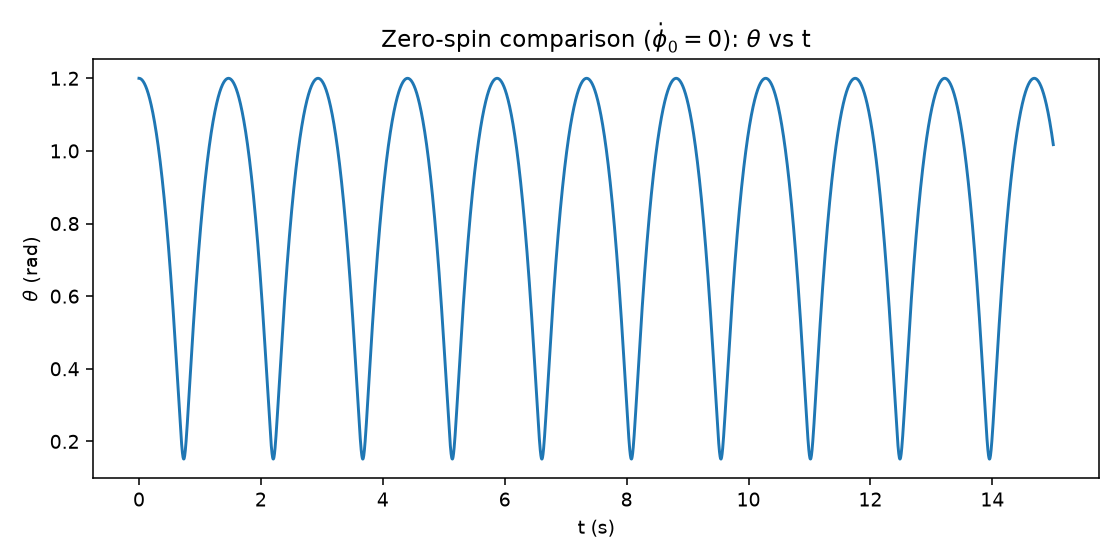
\includegraphics[width=0.75\linewidth]{Figures/Graphs/Problem2/partF_zerospin_theta_vs_t.png}
        \caption{Zero-spin comparison ($\dot\phi_0=0$): $\theta$ nutates periodically (period $\approx1.5$~s) between $0.151$ and $1.2$~rad.}
        \label{fig:zerospin}
    \end{figure}

    Taking instead $\dot\phi_0=6$, the coin nutates about the initial tilt rather than falling toward flat. Running the integration prints
    $$\text{max relative drift in energy } E:\ 1.418\times10^{-12},\qquad \max|\phi_1|,\ \max|\phi_2|:\ 1.104\times10^{-11},\ 1.285\times10^{-11},$$
    confirming energy conservation and that the rolling constraints $\phi_1=\phi_2=0$ are satisfied to numerical precision throughout the integration.

    \begin{figure}[H]
        \centering
        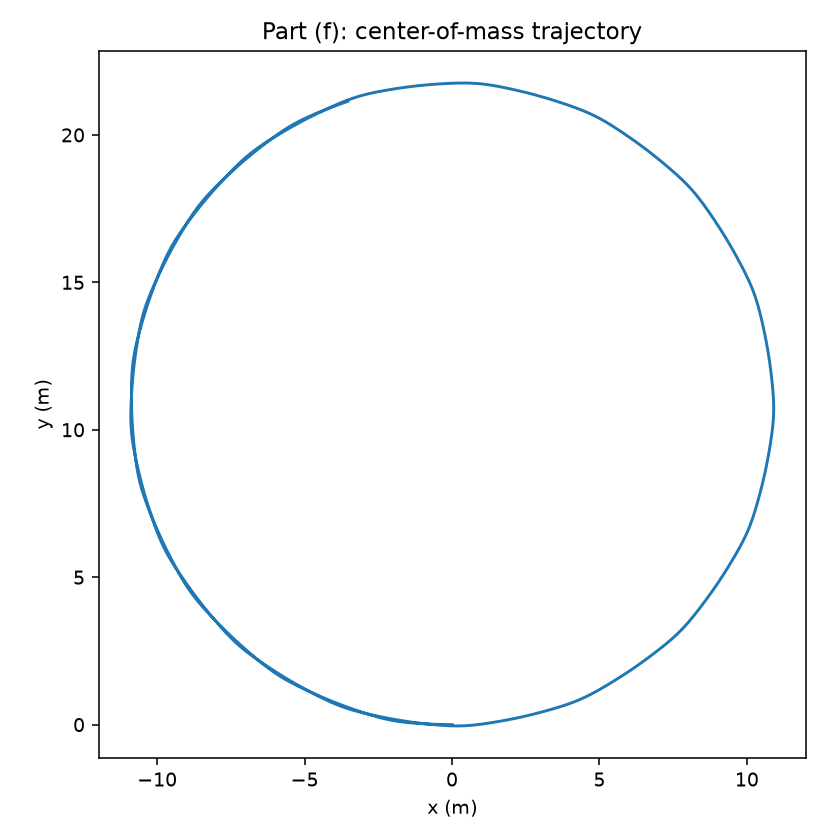
\includegraphics[width=0.6\linewidth]{Figures/Graphs/Problem2/partF_xy_trajectory.png}
        \caption{Part (f): center-of-mass trajectory ($\dot\phi_0=6$).}
    \end{figure}

    \begin{figure}[H]
        \centering
        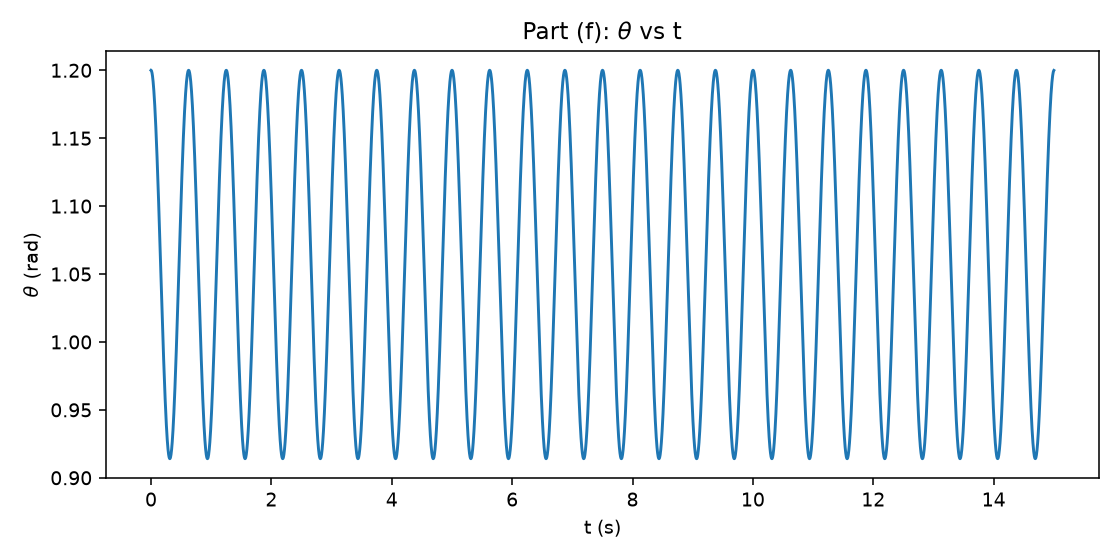
\includegraphics[width=0.75\linewidth]{Figures/Graphs/Problem2/partF_theta_vs_t.png}
        \caption{Part (f): $\theta$ vs.\ $t$ ($\dot\phi_0=6$).}
    \end{figure}

    Nutates between $\theta\approx0.92$ and $1.2$~rad while rolling on a large circular arc of radius $\approx10.9$~m (fit to the trajectory above).

    That radius is worth checking against $v=r(\dot\phi+\dot\psi\cos\theta)$. Doing this with the instantaneous $v(0)\approx6.5$~m/s and the initial rate $\dot\psi_0=1.5$~rad/s is not a valid comparison — $\dot\psi$ oscillates with $\theta$ rather than staying constant, so mixing one instant of $v$ with a different, time-averaged rate isn't a like-for-like check (it happens to land near $4.4$~m, off from the fitted radius by more than a factor of two). The consistent version compares two time-averaged quantities: the total arc length traveled, $\int v\,dt\approx99.0$~m, against the total heading change over the same run, $|\Delta\psi|\approx9.10$~rad, giving $\int v\,dt/|\Delta\psi|\approx10.9$~m — matching the fitted radius of $10.9$~m.

\end{enumerate}

\textit{Note that the transverse moment of inertia for a disk is $I_t=\tfrac14Mr^2$, and the axial moment of inertia is $I_a=\tfrac12Mr^2$.}


% ====================================================
% APPENDIX
% ====================================================
\newpage
\appendix
\section*{Appendix: Code Listings}

\subsection*{Problem 1 Code}
\CodeListing{../code/Problem1.py}{Part (e) phase-portrait integration, sweeping initial conditions above and below $\Omega_{crit}$.}{lst:p1}

\subsection*{Problem 2 Code}
\CodeListing{../code/Problem2.py}{Integrates the coin's equations of motion via the part (e) Lagrange-multiplier system, with energy and constraint checks.}{lst:p2}

\end{document}
